\documentclass[14pt]{extreport}
\usepackage[utf8]{vietnam}
%\usepackage{type1cm}
\usepackage[left=3.50cm, right=2.00cm, top=3.50cm, bottom=3.00cm]{geometry}
%\usepackage[left=3.0cm, right=1.50cm, top=3.00cm, bottom=2.50cm]{geometry}
\usepackage{graphicx}
\usepackage{mathrsfs} 
\usepackage{amsfonts}
\usepackage{longtable}
\usepackage[intlimits]{amsmath}
\usepackage{array}
\usepackage{amsxtra,amssymb,latexsym,amscd,amsthm}
\newtheorem{theorem}{\MakeUppercase{K}ết quả}[section]
% khoảng cách dòng 1.5 lines (như trong MS Word)
\renewcommand{\baselinestretch}{1.5}

%——————–
\begin{document}
%tao khung
\newcommand{\Khung}[2]{
\begin{tabular}{|l|}
\hline\rule[-2ex]{0pt}{5.5ex}
\parbox{#1}{#2}\\
\hline
\end{tabular}
}

\Khung{.92\textwidth}{

\begin{center}
\normalsize
\textbf{TRƯỜNG ĐẠI HỌC BÁCH KHOA HÀ NỘI}\\
\normalsize
\textbf{VIỆN TOÁN ỨNG DỤNG VÀ TIN HỌC}\\
\textbf{------------------------------------------------------}\\[0.4cm]

\includegraphics[scale=.2]{logobkdentrang}\\[1.2cm]
\textbf{{\large NGÔN NGỮ CHÍNH QUY, BIỂU THỨC CHÍNH QUY VÀ SƠ LƯỢC VỀ LÝ THUYẾT MÃ}}\\
\end{center}
\begin{flushleft}
\vspace{1.3cm}
\hspace{1.5cm} \textbf{ Giáng viên hướng dẫn:{ TS. Ngô Thị Hiền }}\\[0.2cm]
\hspace{1.5cm} \textbf{ Nhóm Sinh viên thực hiện:}\\[0.2cm]
\hspace{5cm}\textbf{Nguyễn Anh Tú}\\[0.2cm]
\hspace{5cm}\textbf{Phạm Anh Tuấn}\\[0.2cm]
\hspace{1.5cm} \textbf{ Lớp:\hspace{2cm}{ KSTN Toán Tin K60}}\\
\end{flushleft}

\begin{center}
\textbf{{\small HÀ NỘI - 12/2018}}\\
\end{center}
 }
\thispagestyle{empty}
\newpage

\tableofcontents
\newpage

%\listoffigures

\newpage

\chapter{Giới thiệu}
Ngôn ngữ là phương tiện để giao tiếp, sự giao tiếp có thể hiểu là giao tiếp giữa con người với nhau, giao tiếp giữa người với máy, hay giao tiếp giữa máy với máy. Ngôn ngữ để con người có thể giao tiếp với nhau được gọi là ngôn ngữ tự nhiên, chẳng hạn như tiếng Anh, tiếng Việt… là các ngôn ngữ tự nhiên. Các quy tắc cú pháp của ngôn ngữ tự nhiên nói chung rất phức tạp nhưng các yêu cầu nghiêm ngặt về ngữ nghĩa thì lại thiếu chặt chẽ, chẳng hạn cùng một từ hay cùng một câu ta có thể hiểu chúng theo những nghĩa khác nhau tùy theo từng ngữ cảnh cụ thể. Con người muốn giao tiếp với máy tính tất nhiên cũng thông qua ngôn ngữ. Để có sự giao tiếp giữa người với máy hay giữa máy với nhau, cần phải có một ngôn ngữ với các quy tắc cú pháp chặt chẽ hơn so với các ngôn ngữ tự nhiên, nói cách khác, với một từ hay một câu thì ngữ nghĩa của chúng phải là duy nhất mà không phụ thuộc vào ngữ cảnh. Những ngôn ngữ như thế được gọi là ngôn ngữ hình thức. Con người muốn máy tính thực hiện công việc, phải viết các yêu cầu đưa cho máy bằng ngôn ngữ máy hiểu được. Việc viết các yêu cầu như thế gọi là lập trình. Ngôn ngữ dùng để lập trình được gọi là ngôn ngữ lập trình. Các ngôn ngữ lập trình đều là các ngôn ngữ hình thức. 

Trong bài báo cáo này, nhóm em sẽ trình bày về ngôn ngữ chính quy, biểu thức chính quy và sơ lược về lý thuyết mã.


\chapter{Kiến thức cơ sở}
\section{Xâu}
\begin{itemize}
\item Xâu là một dãy hữu hạn các kí tự 
\item Bảng chữ cái là một tập hợp các kí tự hữu hạn
\item Độ dài xâu là số các kí tự trong xâu đó
\item Xâu rỗng:$\epsilon$, độ dài xâu rồng bằng 0
\item Các phép toán trên xâu:
\begin{enumerate}
\item Ghép nối xâu

Cho 2 xâu:$a=a_1a_2...a_n,b=b_1b_2...b_m$ trên bảng chữ cái $A$. Ghép nối 2 xâu trên ta được một xâu mới $c=ab=a_11_2...a_nb_1b_2...b_m$

Nhận xét: Cho các xâu $s,r,w$ trên bảng chữ cái $A$
\begin{itemize}
\item Xâu rỗng là phần tử đơn vị với phép nối xâu

$s\epsilon =\epsilon s=s$
\item Phép ghép nối có tính chất kết hợp

$\left(sr\right)w=s\left(rw\right)$
\item Kí hiệu $w^n$, với $n$ là số tự nhiên

$w^n=\left\{\begin{matrix}
\epsilon ,n=0\\ 
w,n=1\\ 
w^{n-1}w, n>1
\end{matrix}\right.$
\end{itemize}
\item Xâu con:

$s$ là xâu con của $w$ nếu $\exists s_0,s_1$ sao cho $s_0ss_1=w$

$s_0=\epsilon$ thì $s$ được gọi là prefix của $w$

$s_1=\epsilon$ thì $s$ được gọi là suffix của $w$
\item Phép đảo ngược xâu

$w^R$ được gọi là xâu đảo ngược của $w$ nếu:

$w^{R}=\left\{\begin{matrix}
\epsilon, w=\epsilon \\ 
s_ns_{n-1}...s_0, w=s_0...s_{n-1}s_n; s_i \in A,i=\overline{1,n}
\end{matrix}\right.$

Nhận xét: Cho xâu $s,w$. Phép đảo ngược xâu có các tính chất sau:
\begin{itemize}
\item ${\left(w^R\right)}^R=w$
\item ${\left(sw\right)}^R=w^Rs^R$
\item $\left|w^R\right|=\left|w\right|$
\end{itemize}
\end{enumerate}

\end{itemize}
\section{Ngôn ngữ}
\begin{itemize}
\item Ngôn ngữ là tập các xâu trên bảng chữ cái
\item Các phép toán trên ngôn ngữ

Xét hai ngôn ngữ $L_1,L_2$ trên bảng chữ cái $A$
\begin{enumerate}
\item Phép hợp

Hợp của hai ngôn ngữ $L_1,L_2$, kí hiệu $L_1\cup L_2$ là một ngôn ngữ trên bảng chữ cái $A$:

\begin{center}
$L_1\cup L_2=\{w\in A^*|w\in L_1$ hoặc $ w\in L_2\}$
\end{center}

Định nghĩa phép hợp có thể mở rộng cho hữu hạn các ngôn ngữ:
\begin{center}
$\bigcup_{i=1}^n =\left\{w\in A^*|w\in L_i, i=\overline{1,n}\right\}$
\end{center}

Nhận xét: Xét các ngôn ngữ $L_1,L_2,L_3$.Phép hợp có các tính chất sau
\begin{itemize}
\item Tính chất giao hoán: $L_1\cup L_2=L_2\cup L_1$
\item Tính chất kết hợp: $\left(L_1\cup L_2 \right)\cup L_3=L_1\cup \left(L_2\cup L_3 \right)$
\item $\forall L1:L_1\cup \varnothing =\varnothing \cup L1=L1$ và $L_1 \cup A^*=A^*$
\end{itemize}

\item Phép giao

Giao của hai ngôn ngữ $L_1,L_2$, kí hiệu $L_1\cap L_2$
\begin{center}
$L_1\cap L_2=\{w\in A^*|w\in L_1$ và $ w\in L_2\}$
\end{center}
Định nghĩa phép giao có thể mở rộng cho hữu hạn các ngôn ngữ:
\begin{center}
$\bigcap_{i=1}^n =\left\{w\in A^*|w\in L_i, i=\overline{1,n}\right\}$
\end{center}

Nhận xét: Xét các ngôn ngữ $L_1,L_2,L_3$.Phép hợp có các tính chất sau
\begin{itemize}
\item Tính chất giao hoán: $L_1\cap L_2=L_2\cap L_1$
\item Tính chất kết hợp: $\left(L_1\cap L_2 \right)\cap L_3=L_1\cap \left(L_2\cap L_3 \right)$
\item $\forall L_1:L_1\cap \varnothing =\varnothing \cup L_1=\varnothing$ và $L_1 \cap A^*=L_1$
\item Tính chất phân phối đối với phép hợp và phép giao:
\begin{center}
$\left(L_1\cup L_2\right)\cap L_3=\left(L_1\cap L_3 \right)\cup \left(L_2 \cap L_3\right)$

$\left(L_1\cap L_2\right)\cup L_3=\left(L_1\cup L_3 \right)\cap \left(L_2 \cup L_3\right)$
\end{center}
\end{itemize}
\item Phép nhân ghép

Cho ngôn ngữ $L_1$ trên bảng chữ cái $A_1$, $L_2$ trên bảng chữ cái $A_2$. Phép nhân ghép của hai ngôn ngữ $L_1,L_2$ là một ngôn ngữ trên bảng chữ cái $A_1 \cup A_2$, kí hiệu $L_1L_2$:
\begin{center}
$L_1L_2=\left\{ab|a\in L_1,b\in L_2\right\}$
\end{center}

Nhận xét: Xét các ngôn ngữ $L_1,L_2,L_3$.Phép nhân ghép có các tính chất sau
\begin{itemize}
\item Tính chất kết hợp: $\left(L_1 L_2 \right) L_3=L_1 \left(L_2 L_3 \right)$
\item $\forall L_1:L_1 \varnothing =\varnothing L_1=\varnothing$
\item Tính chất phân phối đối với phép nhân ghép và phép hợp:
\begin{center}
$\left(L_1\cup L_2\right) L_3=\left(L_1 L_3 \right)\cup \left(L_2  L_3\right)$

$L_1\left( L_2\cup L_3\right)=\left(L_1 L_3 \right)\cup \left(L_2 L_3\right)$

\end{center}
\end{itemize}
\end{enumerate}

\item Phép lấy phần bù
Ngôn ngữ phần bù của ngôn ngữ $L$ trên bảng chữ cái $A$, kí hiệu $C_AL$, là một ngôn ngữ trên bảng chữ cái $A$
\begin{center}
$C_AL=\{w\in A^*|w\notin L\}$
\end{center}

Nhận xét:Phép lấy phần bù có các tính chất sau
\begin{itemize}
\item $C_A\{\epsilon \}=A^+,C_AA^+=\{\epsilon \}$
\item $C_A \varnothing =A^*,C_AA^*=\varnothing$
\item $C_A\left(C_AL_1 \cup C_AL_2 \right)=L_1 \cap L_2$
\end{itemize}
\end{itemize}

\section{Ngôn ngữ chính quy}
\subsection{Định nghĩa}

Ngôn ngữ chính quy được định nghĩa như sau:

\begin{enumerate}
\item $\varnothing$ là một ngôn ngữ chính quy
\item $\forall \in A,\left\{a\right\}$ là ngôn ngữ chính quy, $A$: bảng chữ cái
\item $L_1,L_2$ là các ngôn ngữ chính quy thì $L_1 \cup L_2,L_1L_2,L^*$ là các ngôn ngữ chính quy
\item Không có bất kì ngôn ngữ chính quy nào khác ngoài 1,2,3.
\end{enumerate}

\section{Biểu thức chính quy}
\subsection{Định nghĩa}

Biểu thức chính quy được định nghĩa như sau:

\begin{enumerate}
\item $\varnothing$ là biểu thức chính quy
\item $\epsilon$ là biểu thức chính quy
\item $a$ là ngôn ngữ chính quy với $a \in A$, $A$ là bảng chữ cái hữu hạn
\item $r,s$ là biểu thức chính quy

$\left\{\begin{matrix}
(r)(s)\rightarrow RS\\ 
r^{*}\rightarrow R^{*}
\\ (r)+(s)\rightarrow R\cup S

\end{matrix}\right.$ là các biểu thức chính quy
\end{enumerate}
\subsection{Các tính chất của biểu thức chính quy}

Cho $r,s,w$ là các biểu thức chính quy
\begin{enumerate}
\item $r+s=s+r$
\item $\left(r+s\right)+w=r+\left(s+w\right)$
\item $r\left(s+w\right)=rs+rw$
\item $r\epsilon=\epsilon r=r$
\item ${\left(\epsilon+r\right)}^*=r^*$
\item $r+\varnothing=r$
\item ${\left( r^*\right)}^*=r^*$
\item $r+r=r$
\item $r\left(sw\right)=\left(rs\right)w$
\item $\left(r+s\right)w=rw+sw$
\item $\varnothing r=r\varnothing=\varnothing$
\item $\varnothing^*=\epsilon$
\item $r+r^*=r^*$
\item ${\left(r^* s^*\right)}^*={\left(r+s\right)}^*$
\item ${\left(rs\right)}^*r=r{\left(sr\right)}^*$
\end{enumerate}
\subsection{Đồ thị biểu diễn biểu thức chính quy}
\begin{itemize}
\item Mỗi đỉnh là một vòng tròn, đỉnh kết thúc được biểu diễn là một vòng tròn nhân đôi
\item Đỉnh xuất phát thì mũi tên đi vào
\item Các toán tử được biểu diễn như sau:
\begin{center}
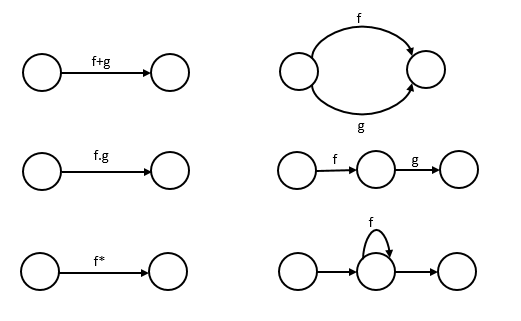
\includegraphics[scale=1.1]{dothibtcq}
\end{center}
\end{itemize}

\section{Automat đơn định(Determinictic Finite Automata)}
\begin{enumerate}
\item Quy luật để chuyển trạng thái mới cho bởi hàm chuyển:

$\delta: Q \times A\rightarrow Q$

$\delta(q,a)=p$

$q,p\in Q,a\in A$
\item Định nghĩa

$M$ là một DFA:
\begin{center}
$M=\left(A,Q,\delta,q_0,F\right)$
\end{center}
Trong đó:
\begin{itemize}
\item $A$: bảng chữ cái hữu hạn
\item $Q$: tập các trạng thái
\item $\delta$: hàm chuyển
\item $q_0$: trạng thái bắt đầu, $q_0 \in Q$
\item $F$: tập trạng thái kết thúc $F\subseteq Q$
\end{itemize}
\end{enumerate}

\section{Automat đa định(Nondeterministic Finite Automata)}
\begin{enumerate}
\item Quy luật để chuyển trạng thái mới cho bởi hàm chuyển:

$\delta: Q \times \left(A\cup \epsilon\right) \rightarrow Q$

$\delta(q,a)=p$

$q,p\in Q,a\in A$
\item Định nghĩa

$M$ là một DFA:
\begin{center}
$M=\left(A,Q,\delta,q_0,F\right)$
\end{center}
Trong đó:
\begin{itemize}
\item $A$: bảng chữ cái hữu hạn
\item $Q$: tập các trạng thái
\item $\delta$: hàm chuyển
\item $q_0$: trạng thái bắt đầu, $q_0 \in Q$
\item $F$: tập trạng thái kết thúc $F\subseteq Q$
\end{itemize}
\end{enumerate}

\section{Văn phạm}
\subsection{Định nghĩa}
Văn phạm $G$ là một bộ gồm 4 thành phần:
$$G = \{ V_T, V_N, S, P \}$$
trong đó:\\
\begin{enumerate}
\item $V_T$ là bảng chữ cái (hay bảng chữ cái kết thúc), mỗi kí tự của nó được gọi là một ký hiệu kết thúc.
\item $V_N$ là bảng chữ cái $V_N \cap V_T = \emptyset$ (hay bảng chữ cái không kết thúc), mỗi phần tử của nó được gọi là một ký hiệu không kết thúc hay ký hiệu phụ
\item $S \in V_N$ được gọi là ký hiệu xuất phát
\item $P$ là tập hợp các luật sinh có dạng $\alpha \rightarrow \beta$, $\alpha$ được gọi là vế trái, còn $\beta$ được gọi là vế phải của một luật sinh, trong đó $\alpha$, $\beta$ $\in (V_N \cup V_T)^*$ và $\alpha$ chứa ít nhất một ký tự không kết thúc.
\end{enumerate}
\subsection{Ngôn ngữ sinh bơi văn phạm}
\textbf{Định nghĩa.} Cho văn phạm $G = \{ V_T, V_N, S, P \}$ và $\eta , \omega \in (V_N \cup V_T)^*$. Ta nói $\omega$ suy dẫn trực tiếp từ $\eta$, ký hiệu $\eta \Rightarrow \omega$, nếu tồn tại luật sinh $\alpha \rightarrow \beta$, và $\gamma , \sigma \in (V_N \cup V_T)^*$ sao cho $\eta = \gamma \alpha \sigma$, $\omega = \gamma \beta \sigma$ \\
\textbf{Định nghĩa.} Cho văn phạm $G = \{ V_T, V_N, S, P \}$ và $\eta , \omega \in (V_N \cup V_T)^*$. Ta nói $\omega$ suy dẫn (hay suy dẫn gián tiếp) từ $\eta$, ký hiệu $\eta \Rightarrow^* \omega$, nếu $\eta = \omega$ hoặc tồn tại một dãy $D = \omega_0 , \omega_1 , ... \omega_k$ sao cho $\omega_0 = \eta$, $\omega_k = \omega$ và $\omega_i \Rightarrow \omega_{i+1}$
\textbf{Định nghĩa.} Cho văm phạm  $G = \{ V_T, V_N, S, P \}$. Xâu $\omega \in V_T^*$ được gọi là sinh bởi văn phạm $G$ nếu tồn tại suy dẫn $S \Rightarrow^* \omega$. Ngôn ngữ sinh bởi văn pham $G$, ký hiệu là $L(G)$, là tập hợp tất cả các xâu sinh bởi văn phạm $G$.
$$L(G) = \{ \omega \in V_N^* | S \Rightarrow^* \omega \}$$

\subsection{Văn phạm chính quy}
Dựa vào đặc điểm của tập luật sinh mà người ta chia các văn phạm thành các nhóm khác nhau. Noam Chomsky đã phân loại văn phạm thành 4 nhóm:
\begin{enumerate}
\item Nhóm 0: Văn phạm không hạn chế
\item Nhóm 1: Văn phạm cảm ngữ cảnh
\item Nhóm 2: Văn phạm phi ngữ cảnh
\item Nhóm 3: Văn phạm chính quy
\end{enumerate}

Trong khuôn khổ của bài báo cáo này, do ta chỉ quan tâm đến ngôn ngữ chính quy, nên bài báo cáo sẽ chỉ trình bày các kết quả liên quan đến văn phạm  chính quy.

\section{Thuật Toán}

\chapter{Sơ lược về lý thuyết mã}
\section{Mã}
$A$ là bảng chữ. $X$ được gọi là mã nếu $\forall m,n$ và $x_1,x_2,...,x_n,y_1,y_2,...,y_m \in X$ thỏa mãn điều kiện:
\begin{center}
$x_1x_2...x_n=y_1y_2...y_m$
\end{center}
Khi đó, $m=n$ và $x_i=y_i,i=\overline{1,n}$
\section{Mã tối đại}
Mã $X$ được gọi là tối đại trên $A$ nếu $X$ không chứa thực sự trong một mã nào khác trên $A$.

Với mỗi lớp mã $C$ trên $A$, một mã $X\in C$ là tối đại trong $C$($C$ không nhất thiết là mã tối đại) nếu nó không chứa thực sự trong một mã nào khác của $C$.
\section{Mã prefix}
	Cho tập $X$ là tập con của $A^*$. $X$ được gọi là mã prefix nếu không có phần tử nào trên $X$ nằm ở bên trái của một phần tử khác trong $X$

Nói cách khác, X là prefix nếu với mọi $x,x' \in X: x\leq x' \Rightarrow x=x'$

\section{Tiêu chuẩn kiểm định mã}
Bài toán:
\begin{itemize}
\item Input: 1 ngôn ngữ chính quy
\item Output: Có phải là mã không?
\end{itemize}
Cho $X\subseteq A^+: U_1=X^{-1}X-\{\epsilon\},...;U_{n+1}=X^{-1}U_n \cup U_n^{-1}X$ với $n\geq 1$
\begin{itemize}
\item Mệnh đề: Nếu $X$ là một ngôn ngữ chính quy thì tập tất cả các $U_n$ là hữu hạn với $n\geq 1$

\item Điều kiện dừng của thuật toán:

Nếu $\epsilon \in U_i $ thì X không phải là mã

Nếu $U_i=U_n$ hoặc $U_n=\varnothing$ thì X là mã
\end{itemize}

\chapter{Ứng dụng: Single-Error Correcting Codes}




\chapter{Kết luận}
{\huge \textbf{Tài liệu tham khảo}}
\end{document}
